\documentclass{tufte-handout}

\usepackage{hyperref} % hyperlinks
	\hypersetup{colorlinks}
\usepackage{tikz}     % block diagrams
	\usetikzlibrary{matrix}
\usepackage{amsmath}  % extended mathematics

\title{Current-Mode Control Small-Signal Model\thanks{\href{https://ridleyengineering.com/images/current_mode_book/CurrentModeControl.pdf}{Original derivations by Dr. Raymond B. Ridley of Ridley Engineering.}}}

\author[Alexander Osborne]{Alexander Osborne}

\begin{document}

\maketitle

\begin{abstract}
\noindent
This document seeks to clarify the block diagrams and equations presented in Dr. Raymond B. Ridley's PhD dissertation, "A New Small-Signal Model for Current-Mode Control."
All equations presented herein are as applied to a buck converter with constant-frequency, trailing-edge peak current-mode control.
\end{abstract}

\section{Small-Signal Block Diagram}

\begin{fullwidth}
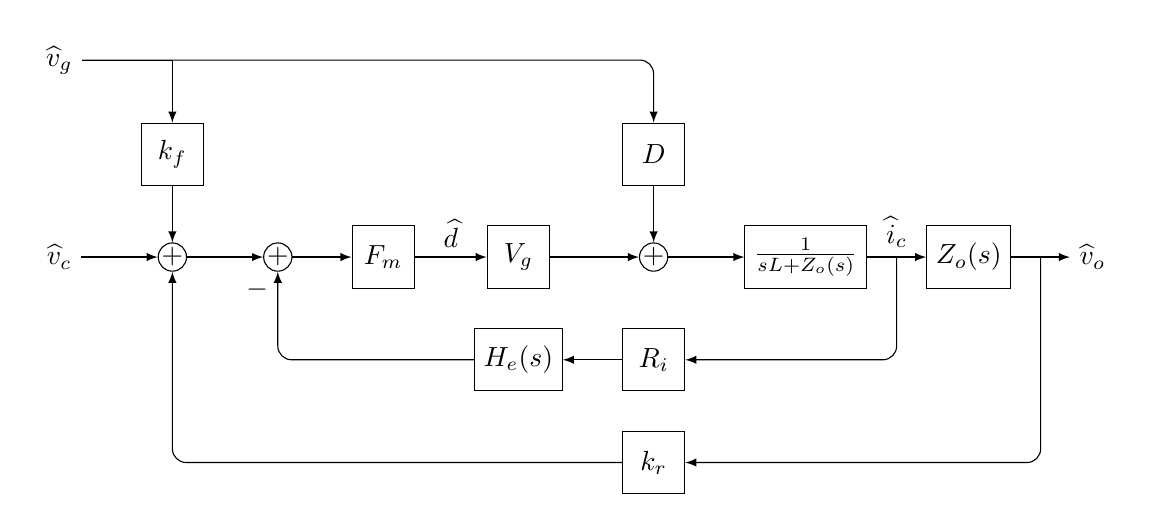
\begin{tikzpicture}[auto,
                    >=latex,
                    block/.style={draw, rectangle, align=center, minimum height=2.25em, minimum width=2.25em},
                    circ/.style={draw, circle, align=center, inner sep=0pt, minimum size=1em},
                    ra/.style={->, rounded corners=0.5em}]

\matrix[column sep=0.75cm, row sep=0.5cm]{

\node (vghat) {$\widehat{v}_g$}; \\

& \node [block] (kf) {$k_f$}; & & & & 
\node [block] (D) {$D$}; \\

\node (vchat) {$\widehat{v}_c$}; &
\node [circ] (c21) {$+$}; &
\node [circ] (c22) {$+$}; &
\node [block] (Fm) {$F_m$}; &
\node [block] (Vg) {$V_g$}; &
\node [circ] (c25) {$+$}; &
\node [block] (sL) {$\frac{1}{sL+Z_o(s)}$}; &
\node [block] (Zo) {$Z_o(s)$}; &
\node (vohat) {$\widehat{v}_o$}; \\

& & & & \node [block] (He) {$H_e(s)$}; &
\node [block] (Ri) {$R_i$}; \\

& & & & & \node [block] (kr) {$k_r$}; \\};

\draw [ra] (vghat) -| (D);
\draw [->] (vghat) -| (kf);
\draw [->] (kf) -- (c21);
\draw [->] (vchat) -- (c21);
\draw [->] (D) -- (c25);
\draw [->] (c21) -- (c22);
\draw [->] (c22) -- (Fm);
\draw [->] (Fm) -- node {$\widehat{d}$} (Vg);
\draw [->] (Vg) -- (c25);
\draw [->] (c25) -- (sL);
\draw [->] (sL) -- node[name=ic] {$\widehat{i}_c$} (Zo);
\draw [->] (Zo) -- node[name=vo] {} (vohat);
\draw [ra] (ic) |- (Ri);
\draw [->] (Ri) -- (He);
\draw [ra] (He) -| node[pos=0.9] {$-$} (c22);
\draw [ra] (kr) -| (c21);
\draw [ra] (vo) |- (kr);
\end{tikzpicture}
\end{fullwidth}

\marginnote[2em]{$V_g$ \ \ steady-state input voltage}
\marginnote{$V_o$ \ \ steady-state output voltage}
\marginnote{$D=V_o/V_g$ \ \ steady-state duty cycle}
\marginnote{$\widehat{v}_g$ \ \ small-signal input voltage}
\marginnote{$\widehat{v}_o$ \ \ small-signal output voltage}
\marginnote{$\widehat{d}$ \ \ small-signal duty cycle}
\marginnote{$\widehat{i}_c$ \ \ small-signal inductor current}
\marginnote{$\widehat{v}_c$ \ \ small-signal control voltage}
\marginnote{$sL$ \ \ inductor impedance}
\marginnote{$Z_o(s)$ \ \ output impedance}
\marginnote{$R_i$ \ \ sense resistor}
\marginnote{$H_e(s)$ \ \ sample-and-hold effect}
\marginnote{$F_m$ \ \ modulation gain}
\marginnote{$k_f$ \ \ input feed-forward gain}
\marginnote{$k_r$ \ \ output feed-forward gain}
\marginnote{$S_e$ \ \ slope compensation ramp}
\marginnote{$S_n=(V_g-V_o)R_i/L$ \ \ on-time ramp}
\marginnote{$S_f=V_oR_i/L$ \ \ off-time ramp}
\marginnote{$T_s$ \ \ switching period}

Dr. Ridley's diagrams generally mix transfer function blocks with circuit element symbols.
As an alternative, a complete transfer function block diagram is provided above.
Transfer function descriptions and key parameter definitions are in the margins.
\begin{align*}
F_m&=\frac{1}{(S_n+S_e)T_s}\\[0.75em]
H_e(s)&=1-s\frac{T_s}{2}+s^2\left(\frac{T_s}{\pi}\right)^2\\[0.75em]
k_f&=\frac{-DT_sR_i}{L}\left(1-\frac{D}{2}\right)\\[0.75em]
k_r&=\frac{T_sR_i}{2L}
\end{align*}

Multiple forms of the modulation gain $F_m$ can be found in literature; their differences stem from how the average inductor current is defined relative to the peak.
Dr. Ridley has experimentally verified the modulation gain used in this model is correct.

$H_e(s)$ is an approximation that is only valid up to one-half the switching frequency.
Such an approximation will suffice because a stable system must have a crossover frequency beneath the Nyquist frequency of the system.

In order to simplify the design of the outer voltage loop feedback compensation network, a transfer function from the duty cycle to inductor current $F_i$ can be defined that is independent of the output impedance $Z_o(s)$.
Such a transfer function will only be valid for frequencies where $Z_o(s) \ll sL$. Assuming the output impedance is predominantly capacitive, this transfer function would apply above the resonant frequency.
\begin{align*}
F_i&=\frac{\widehat{i}_c}{\widehat{d}}=\frac{V_g}{sL+Z_o(s)}\approx\frac{V_g}{sL}=\frac{S_n+S_f}{sR_i}\\[0.75em]
\alpha&=\frac{S_f-S_e}{S_n+S_e}\\[0.75em]
F_mF_i&\approx\frac{1+\alpha}{sR_iT_s}
\end{align*}

The output voltage feed-forward gain $k_r$ can be ignored unless analyzing the low frequency gain of a converter operating near discontinuous conduction mode. The transfer function from the control voltage to inductor current $F(s)$ then becomes rather simple.
\begin{align*}
F(s)=\frac{\widehat{i}_c}{\widehat{v}_c}&=\frac{F_mV_g}{sL+Z_o(s)+F_mV_g(R_iH_e(s)-k_rZ_o(s))}\\[0.75em]
&\approx\frac{F_mF_i}{1+F_mF_iR_iH_e(s)}
\end{align*}

\section{Closed-Loop Design Procedure}

\begin{fullwidth}
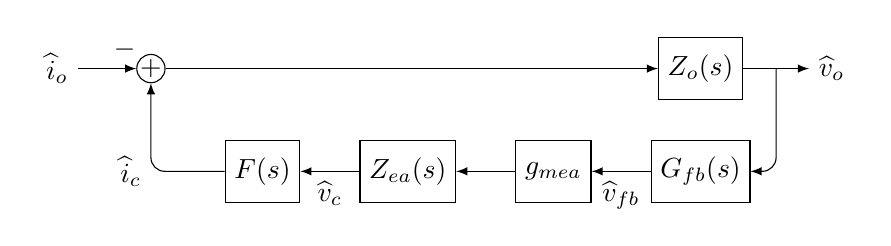
\begin{tikzpicture}[auto,
                    >=latex,
                    block/.style={draw, rectangle, align=center, minimum height=2.25em, minimum width=2.25em},
                    circ/.style={draw, circle, align=center, inner sep=0pt, minimum size=1em},
                    ra/.style={->, rounded corners=0.5em}]

\matrix[column sep=0.75cm, row sep=0.5cm]{

\node (iohat) {$\widehat{i}_o$}; &
\node [circ] (c01) {$+$}; & & & &
\node [block] (Zo) {$Z_o(s)$}; &
\node (vohat) {$\widehat{v}_o$}; \\

& & \node [block] (Fs) {$F(s)$}; &
\node [block] (Zea) {$Z_{ea}(s)$}; &
\node [block] (gmea) {$g_{mea}$}; &
\node [block] (Gfb) {$G_{fb}(s)$}; \\};

\draw [->] (iohat) -- node[pos=0.8] {$-$} (c01);
\draw [->] (c01) -- (Zo);
\draw [->] (Zo) -- node[name=vo] {} (vohat);
\draw [->] (Gfb) -- node[name=vfb] {$\widehat{v}_{fb}$} (gmea);
\draw [->] (gmea) -- (Zea);
\draw [->] (Zea) -- node[name=vc] {$\widehat{v}_c$} (Fs);
\draw [ra] (Fs) -| node[name=ic] {$\widehat{i}_c$} (c01);
\draw [ra] (vo) |- (Gfb);

\end{tikzpicture}
\end{fullwidth}

A typical network to close the loop around $F(s)$ is shown above. The load is assumed to be an ideal current sink $\widehat{i}_o$.
The output voltage passes through the feedback network $G_{fb}(s)$ and is compared against a fixed reference voltage.
A transconductance error amplifier $g_{mea}$ is loaded by the error amplifier compensation network $Z_{ea}(s)$ to generate the control voltage.

The loop gain $T(s)$ is designed for the appropriate stability margin.
The step response is derived from the closed-loop transfer function $Y(s)$.
\begin{align*}
T(s)&=F(s)Z_o(s)G_{fb}(s)g_{mea}Z_{ea}(s)\\[0.75em]
Y(s)&=\frac{\widehat{v}_o}{\widehat{i}_o}=\frac{Z_o(s)}{T(s)-1}=\frac{Z_o(s)}{F(s)Z_o(s)G_{fb}(s)g_{mea}Z_{ea}(s)-1}
\end{align*}

An iterative design procedure will yield good results.
In general, reducing $Z_o(s)$ and increasing the gain and bandwidth of $T(s)$ will yield a step response with less overshoot and faster settling time.
\begin{enumerate}
\item Select a ripple current relative to the maximum load current, 10\% to 30\% is typical.
Select a switching frequency and inductance $L$.
Design $Z_o(s)$ to have low impedance at the switching frequency to meet the required voltage ripple.
\item Use the approximate form of $F(s)$ to design $Z_o(s)$, $G_{fb}(s)$, and $Z_{ea}(s)$ to stabilize the loop gain.
This will require an initial guess for the required low frequency impedance of $Z_o(s)$. $G_{fb}(s)Z_{ea}(s)$ must, at a minimum, be a Type-II network.
\item Use the exact form of $F(s)$ to simulate the closed-loop step response. Iterate the design of $Z_o(s)$, $G_{fb}(s)$, and $Z_{ea}(s)$ to achieve the desired step response.
\end{enumerate}

\end{document}